\subsection{Measurable Functions}

% **Role:** modern integration and almost-everywhere analysis.
%
% Measurable maps, simple functions, convergence almost everywhere, convergence in measure.

\begin{definition} \label{def:measure-space-and-measurable-functions} \hlt{Borel, Lebesgue, and Function Measurability}
\begin{enumerate}[label=(\roman*)]
\setlength{\itemsep}{0pt}
\item \hlt{Borel}: $\mathcal{B}(\R^p)\defeq\sigma(\mathcal{O}_{\R^p})$; its elements are \hlt{Borel sets}.
\item \hlt{Lebesgue}: $\mathcal{B}(\R^p)\subseteq\mathcal{L}^p$, and $\mathcal{L}^p$ is obtained by adjoining subsets of Lebesgue null sets.
\item \hlt{Maps}: for measurable spaces $(X,\mathcal{M})$, $(Y,\mathcal{N})$, $f:X\to Y$ is \hlt{$(\mathcal{M},\mathcal{N})$-measurable} iff $\forall E\in\mathcal{N},\ f^{-1}(E)\in\mathcal{M}$.
\item \hlt{Borel maps}: $f:\R^p\to\R^q$ is \hlt{Borel measurable} iff $\forall B\in\mathcal{B}(\R^q),\ f^{-1}(B)\in\mathcal{B}(\R^p)$.
\item \hlt{Thresholds}: write $\{f\bowtie a\}\defeq\{x\in X:f(x)\bowtie a\}$ for $\bowtie\in\{>,\geq,<,\leq\}$.\\
Extended-real $f$ is \hlt{$\mathcal{M}$-measurable} iff $\forall a\in\R,\ \{f>a\}\in\mathcal{M}$.
\end{enumerate}
\hlt{Structural Commentary}: Borel measurability tracks topology; Lebesgue measurability adds null-set completion.\\
\hlt{Key Insight}: Measurability is inverse-image stability.
\end{definition}

\begin{proposition} \label{prop:measurable-map-generator-test} \hlt{Generator Test for Measurable Maps}\\
Let $f:X\to Y$, $\mathcal{A}\subseteq\mathcal{P}(Y)$, and $\mathcal{N}\defeq\sigma(\mathcal{A})$.
\begin{enumerate}[label=(\roman*)]
\setlength{\itemsep}{0pt}
\item If $\forall A\in\mathcal{A},\ f^{-1}(A)\in\mathcal{M}$, then $f:X\to(Y,\mathcal{N})$ is measurable.
\item For real-valued $f$, $\forall a\in\R,\ \{f>a\}\in\mathcal{M}\Longleftrightarrow \forall B\in\mathcal{B}(\R),\ f^{-1}(B)\in\mathcal{M}$.
\end{enumerate}
\begin{proof}
\begin{enumerate}[label=(\roman*)]
\setlength{\itemsep}{0pt}
\item Let $\mathcal{G}\defeq\{E\subseteq Y:f^{-1}(E)\in\mathcal{M}\}$. Since $f^{-1}(E^c)=f^{-1}(E)^c$ and $f^{-1}(\bigcup\limits_nE_n)=\bigcup\limits_nf^{-1}(E_n)$, $\mathcal{G}$ is a $\sigma$-algebra. Thus $\mathcal{A}\subseteq\mathcal{G}\Longrightarrow\mathcal{N}=\sigma(\mathcal{A})\subseteq\mathcal{G}$.
\item[$(ii)$] ($\Rightarrow$) Set $\mathcal{A}\defeq\{(a,+\infty):a\in\R\}$. Since $\forall a\in\R,\ f^{-1}((a,+\infty))=\{f>a\}\in\mathcal{M}$ and $\sigma(\mathcal{A})=\mathcal{B}(\R)$, (i) gives $\forall B\in\mathcal{B}(\R),\ f^{-1}(B)\in\mathcal{M}$.
\item[$(ii)$] ($\Leftarrow$) If $\forall B\in\mathcal{B}(\R),\ f^{-1}(B)\in\mathcal{M}$, then $\forall a\in\R,\ \{f>a\}=f^{-1}((a,+\infty))\in\mathcal{M}$.
\end{enumerate}
\hlt{Structural Commentary}: Measurability can be checked on any generating family of target sets.\\
\hlt{Key Insight}: Pullbacks turn generated $\sigma$-algebras into generated collections of preimages.
\end{proof}
\end{proposition}

\begin{proposition} \label{prop:measurable-function-open-set-test} \hlt{Open-Set Test for Euclidean Targets}\\
Let $\Omega\subseteq\R^n$ be Lebesgue measurable and let $f:\Omega\to\R^m$. The following tests are equivalent:
\begin{enumerate}[label=(\roman*)]
\setlength{\itemsep}{0pt}
\item $\forall V\subseteq\R^m$ open, $f^{-1}(V)$ is measurable;
\item $\forall B\subseteq\R^m$ open boxes, $f^{-1}(B)$ is measurable;
\item $\forall j\in\{1,\ldots,m\}$, $f_j:\Omega\to\R$ is threshold-measurable.
\end{enumerate}
In particular, every continuous $f:\Omega\to\R^m$ is measurable.
\begin{proof}
\begin{enumerate}[label=(\roman*).]
\setlength{\itemsep}{0pt}
\item[$(i)$]$\Rightarrow (ii)$. Open boxes are open.
\item[$(ii)$]$\Rightarrow (i)$. By Lemma \ref{lem:open-sets-countable-unions-rational-boxes}, $V=\bigcup\limits_kB_k$ for rational boxes $B_k$, hence $f^{-1}(V)=\bigcup\limits_kf^{-1}(B_k)$ is measurable.
\item[$(ii)$]$\Rightarrow (iii)$. By $(ii)\Rightarrow(i)$, $\{f_j>a\}=f^{-1}(\{y:y_j>a\})$ is measurable.
\item[$(iii)$]$\Rightarrow (ii)$. If $B=\prod\limits_{j=1}^{m}(a_j,b_j)$, then $f^{-1}(B)=\bigcap\limits_{j=1}^{m}\bigl(\{f_j>a_j\}\cap\{f_j<b_j\}\bigr)$,\\
where $\{f_j<b_j\}=\Omega\setminus\bigcap\limits_{\ell=1}^{\infty}\{f_j>b_j-\frac{1}{\ell}\}$. Thus each factor is measurable, hence so is $f^{-1}(B)$.
\end{enumerate}
If $f$ is continuous, $f^{-1}(V)$ is open relative to $\Omega$ by Theorem \ref{thm:continuity-open-preimages}.\\
By Theorem \ref{thm:relative-open-intersection-with-open-set}, $f^{-1}(V)=W\cap\Omega$ for some open $W\subseteq\R^n$, hence it is measurable by Theorem \ref{thm:lebesgue-measure-basic-properties-checklist}.\\
\hlt{Structural Commentary}: Euclidean-valued measurability is just countable box algebra applied to inverse images.\\
\hlt{Key Insight}: Open sets reduce to rational boxes; vector functions reduce to coordinate threshold tests.
\end{proof}
\end{proposition}

\begin{example} \label{ex:basic-measurable-functions} \hlt{Basic Measurable Functions}\\
Let $(X,\mathcal{M})$ be a measurable space.
\begin{enumerate}[label=(\roman*)]
\setlength{\itemsep}{0pt}
\item Constant real-valued functions are measurable, since each strict superlevel set is either $X$ or $\emptyset$.
\item For $E\subseteq X$, the indicator $\mathbf{1}_E$ is measurable iff $E\in\mathcal{M}$.
\item Continuous maps between Euclidean measurable subsets are measurable by Proposition \ref{prop:measurable-function-open-set-test}.
\item Monotone functions $\R\to\R$ are Borel measurable, since their strict superlevel sets are half-lines, $\R$, or $\emptyset$.
\end{enumerate}
\hlt{Key Insight}: Constants, indicators of measurable sets, continuous functions, and monotone functions form the first reusable stock of measurable functions.
\end{example}

\begin{theorem} \label{thm:measurable-function-closure} \hlt{Closure Properties of Measurable Functions}\\
Let $(X,\mathcal{M})$ be a measurable space.
\begin{enumerate}[label=(\roman*)]
\setlength{\itemsep}{0pt}
\item The four tests $\forall a\in\R,\ \{f>a\},\{f\geq a\},\{f<a\},\{f\leq a\}\in\mathcal{M}$ are equivalent.
\item $f$ measurable implies $\abs{f}$ measurable.
\item If $f_n$ are measurable, then $\sup\limits_nf_n,\inf\limits_nf_n,\limsup\limits_nf_n,\liminf\limits_nf_n$ are measurable.
\item If $f,g$ real-valued measurable, $F:\R^2\to\R$ continuous, then $F(f,g)$ measurable; so are $f+g$ and $fg$.
\end{enumerate}
\begin{proof}
\begin{enumerate}[label=(\roman*)]
\setlength{\itemsep}{0pt}
\item Use $\{f\geq a\}=\bigcap\limits_{m\geq1}\{f>a-\frac{1}{m}\}$; $\{f<a\}=X\setminus\{f\geq a\}$; $\{f\leq a\}=\bigcap\limits_{m\geq1}\{f<a+\frac{1}{m}\}$.
\item For $a>0$, $\{\abs{f}<a\}=\{f<a\}\cap\{f>-a\}$; for $a\leq0$ the set is empty.
\item $\{\sup\limits_nf_n>a\}=\bigcup\limits_n\{f_n>a\}$. Also $\limsup\limits_nf_n=\inf\limits_m\sup\limits_{n\geq m}f_n$; $\liminf\limits_nf_n=\sup\limits_m\inf\limits_{n\geq m}f_n$; inf follow from (i).
\item For $G_a=\{(u,v):F(u,v)>a\}$, write $G_a=\bigcup\limits_k(\alpha_k,\beta_k)\times(\gamma_k,\delta_k)$.\\
Then $\{F(f,g)>a\}=\bigcup\limits_k\bigl(\{\alpha_k<f<\beta_k\}\cap\{\gamma_k<g<\delta_k\}\bigr)\in\mathcal{M}$.
\end{enumerate}
\hlt{Structural Commentary}: Measurability is countable set algebra applied to level sets.\\
\hlt{Key Insight}: Once threshold sets are measurable, ordinary limiting and algebraic operations stay measurable.
\end{proof}
\end{theorem}

\begin{corollary} \label{cor:continuous-composition-and-finite-lattice-measurable} \hlt{Continuous Composition and Finite Lattice Operations}\\
Let $(X,\mathcal{M})$ be a measurable space and let $n\in\mathbb{N}_{\geq1}$.\\
For $f_1,\ldots,f_n:X\to\R$, set $\bigvee_{k=1}^{n}f_k\defeq\max\{f_1,\ldots,f_n\}$ and $\bigwedge_{k=1}^{n}f_k\defeq\min\{f_1,\ldots,f_n\}$.
\begin{enumerate}[label=(\roman*)]
\setlength{\itemsep}{0pt}
\item If $g:X\to\R$ is measurable and $\varphi:\R\to\R$ is continuous, then $\varphi\circ g$ is measurable.
\item If $f_1,\ldots,f_n:X\to\R$ are measurable, then $\bigvee_{k=1}^{n}f_k$ and $\bigwedge_{k=1}^{n}f_k$ are measurable.
\end{enumerate}
\begin{proof}
\begin{enumerate}[label=(\roman*)]
\setlength{\itemsep}{0pt}
\item For $a\in\R$, $\{\varphi\circ g>a\}=g^{-1}(\varphi^{-1}((a,+\infty)))\in\mathcal{M}$, since $\varphi^{-1}((a,+\infty))\in\mathcal{B}(\R)$ and $g$ is measurable.
\item Set $h_k=f_k$ for $1\leq k\leq n$ and $h_k=f_n$ for $k>n$. Then $(h_k)$ is measurable, $\bigvee_{k=1}^{n}f_k=\sup\limits_{k\geq1}h_k$, and $\bigwedge_{k=1}^{n}f_k=\inf\limits_{k\geq1}h_k$, hence both are measurable by Theorem \ref{thm:measurable-function-closure}(iii).
\end{enumerate}
\hlt{Structural Commentary}: Pullbacks preserve Borel thresholds; finite lattices are finite suprema and infima.\\
\hlt{Key Insight}: Continuity and finite lattice operations preserve measurable threshold structure.
\end{proof}
\end{corollary}

\begin{example} \label{ex:measurable-composition-can-fail} \hlt{Measurable Composition Can Fail}\\
Choose $A\in\mathcal{L}^1$ with $A\subseteq[0,1]$ and an increasing homeomorphism $\psi:[0,1]\to[0,2]$ such that $\psi(A)\notin\mathcal{L}^1$. Define
\begin{equation*}
\widetilde{\psi}(x)\defeq
\begin{cases}
x,&x\leq0,\\
\psi(x),&0\leq x\leq1,\\
x+1,&x\geq1.
\end{cases}
\end{equation*}
Then $\widetilde{\psi}:\R\to\R$ is a homeomorphism. Put $h\defeq\mathbf{1}_A\circ\widetilde{\psi}^{-1}$.\\
The maps $\mathbf{1}_A$ and $\widetilde{\psi}^{-1}$ are measurable, but $h^{-1}((\frac{1}{2},\frac{3}{2}))=\widetilde{\psi}(A)=\psi(A)\notin\mathcal{L}^1$.\\
Hence $h$ is not Lebesgue measurable, so Lebesgue measurable functions are not composition-closed.
\end{example}

\begin{definition} \label{def:positive-negative-parts-measurable-functions} \hlt{Positive and Negative Parts}\\
For an extended-real-valued function $f$, define $f^+(x)\defeq\sup\{f(x),0\}$; $f^-(x)\defeq\sup\{-f(x),0\}$.\\
When $f$ is finite-valued, $f=f^+-f^-$ and $\abs{f}=f^++f^-$; equivalently $f^+=\frac{\abs{f}+f}{2}$; $f^-=\frac{\abs{f}-f}{2}$.
\end{definition}

\begin{corollary} \label{cor:positive-negative-parts-measurable} \hlt{Measurability of Positive and Negative Parts}\\
If $f:X\to[-\infty,+\infty]$ is measurable, then $f^+,f^-,\abs{f}$ are measurable.\\
If $f:X\to\R$, then $f$ measurable $\Longleftrightarrow$ $f^+,f^-$ measurable.
\begin{proof}
\begin{enumerate}[label=\roman*.]
\setlength{\itemsep}{0pt}
\item[$(\Rightarrow)$] Since $\{-f>a\}=\{f<-a\}$, $-f$ is measurable.\\
Thus $f^+=f\vee0$, $f^-=(-f)\vee0$, and $\abs{f}=f\vee(-f)$ are measurable by finite sup-closure.
\item[$(\Leftarrow)$] If $f:X\to\R$ and $f^+,f^-$ are measurable, then $f=f^+-f^-$ is measurable.
\end{enumerate}
\hlt{Structural Commentary}: Sign decomposition is compatible with threshold-set measurability.\\
\hlt{Key Insight}: Reduce signs to suprema and finite algebra.
\end{proof}
\end{corollary}

\begin{lemma} \label{lem:extended-real-measurable-finite-part} \hlt{Extended-Valued Measurability via the Finite Part}\\
Let $f:X\to\overline{\R}$ and set $A\defeq f^{-1}(\{+\infty\})$, and $B\defeq f^{-1}(\{-\infty\})$.
Define $f_0(x)\defeq
\begin{cases}
f(x),&x\notin A\cup B,\\
0,&x\in A\cup B.
\end{cases}$.\\
Then $f$ is measurable iff $A,B\in\mathcal{M}$ and $f_0:X\to\R$ is measurable.
\begin{proof}
\begin{enumerate}[label=\roman*.]
\setlength{\itemsep}{0pt}
\item[$(\Rightarrow)$] If $f$ is measurable, then $A=\bigcap\limits_{n=1}^{\infty}\{f>n\}$; and $B=X\setminus\bigcup\limits_{n=1}^{\infty}\{f>-n\}$, so $A,B\in\mathcal{M}$.\\
Also, $\{f_0>\alpha\}=
\begin{cases}
\{f>\alpha\}\setminus A,&\alpha\geq0,\\
\{f>\alpha\}\cup B,&\alpha<0,
\end{cases}$, so $f_0$ is measurable.
\item[$(\Leftarrow)$] If $A,B\in\mathcal{M}$, $f_0$ is measurable, then $\{f>\alpha\}=
\begin{cases}
\{f_0>\alpha\}\cup A,&\alpha\geq0,\\
\{f_0>\alpha\}\setminus B,&\alpha<0,
\end{cases}$, so $\{f>\alpha\}\in\mathcal{M}$ $\forall \alpha\in\R$.
\end{enumerate}
\hlt{Structural Commentary}: The infinite-level sets are measurable exactly when the finite core is measurable.\\
\hlt{Key Insight}: Assign harmless finite values at $\pm\infty$, then put the infinite fibers back by set algebra.
\end{proof}
\end{lemma}

\begin{corollary} \label{cor:extended-measurable-algebra-conventions} \hlt{Extended-Valued Algebra Conventions}\\
Let $f,g:X\to\overline{\R}$ be measurable.
\begin{enumerate}[label=(\roman*)]
\setlength{\itemsep}{0pt}
\item For $c\in\R$, $cf$, $\abs{f}$, $f^+$, and $f^-$ are measurable, with $0(\pm\infty)=0$.
\item Let $E_1\defeq\{f=-\infty,\ g=+\infty\}$, $E_2\defeq\{f=+\infty,\ g=-\infty\}$, and $F\defeq E_1\cup E_2$.\\
If $h=f+g$ on $X\setminus F$ and $h=0$ on $F$, then $h$ is measurable.
\item With $0(\pm\infty)=0$, $fg$ is measurable.
\end{enumerate}
\begin{proof}
\begin{enumerate}[label=(\roman*)]
\setlength{\itemsep}{0pt}
\item By Lemma \ref{lem:extended-real-measurable-finite-part}, $A_\pm(f)\defeq\{f=\pm\infty\}\in\mathcal{M}$ and $f_0$ is measurable.\\
For $c\in\R$, the infinite fibers of $cf$ are among $A_\pm(f)$ and $(cf)_0=cf_0$, so $cf$ is measurable.\\
The functions $\abs{f},f^+,f^-$ are measurable by Corollary \ref{cor:positive-negative-parts-measurable}.
\item $E_1,E_2\in\mathcal{M}$. Set $f_n\defeq\max\{-n,\min(f,n)\}$ and $g_n\defeq\max\{-n,\min(g,n)\}$.\\
Then $f_n,g_n$ are real-valued measurable and $(f_n+g_n)\mathbf{1}_{X\setminus F}\to h$ pointwise; hence $h$ is measurable.
\item With $f_n,g_n$ as in (ii), $f_ng_n$ measurable, $f_ng_n\to fg$ pointwise under $0(\pm\infty)=0$; hence $fg$ measurable.
\end{enumerate}
\hlt{Structural Commentary}: Extended algebra is finite algebra plus measurable exceptional fibers.\\
\hlt{Key Insight}: Truncate first, use real-valued closure, then pass to pointwise limits.
\end{proof}
\end{corollary}

\begin{definition} \label{def:simple-functions-measurable} \hlt{Simple Functions}\\
Let $(X,\mathcal{M})$ be a measurable space.
\begin{enumerate}[label=(\roman*)]
\setlength{\itemsep}{0pt}
\item \hlt{Indicator}: for $E\subseteq X$, $\mathbf{1}_E(x)\defeq1$ on $E$ and $\mathbf{1}_E(x)\defeq0$ on $X\setminus E$.
\item \hlt{Simple}: a real-valued $s$ is simple iff $s(X)$ is finite.
\item \hlt{Standard representation}: if $s(X)=\{c_1,\ldots,c_n\}$ and $E_i\defeq\{s=c_i\}\neq\emptyset$, then $X=\bigsqcup\limits_{i=1}^{n}E_i$; $s=\sum\limits_{i=1}^{n}c_i\mathbf{1}_{E_i}$.\\
The pairs $(c_i,E_i)$ are unique up to reordering.
\item \hlt{Measurability}: $s$ measurable iff $E_i\in\mathcal{M}$ $\forall i$; step functions are special case $X\subseteq\R$ with interval level sets.
\end{enumerate}
\end{definition}

\begin{figure}[H]
  \centering
  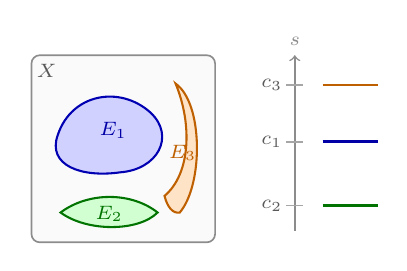
\begin{tikzpicture}[
  scale=0.88,
  every node/.style={font=\scriptsize},
  setbox/.style={draw=black!45, fill=black!2, line width=0.6pt, rounded corners=3pt},
  piecea/.style={fill=blue!18, draw=blue!70!black, line width=0.75pt},
  pieceb/.style={fill=green!18, draw=green!45!black, line width=0.75pt},
  piecec/.style={fill=orange!22, draw=orange!75!black, line width=0.75pt},
  axis/.style={->, black!45, line width=0.55pt},
  tick/.style={draw=black!35, line width=0.5pt},
  value/.style={line width=1.0pt}
]
  \draw[setbox] (-3.0,-1.35) rectangle (-0.35,1.35);
  \node[black!65] at (-2.78,1.12) {$X$};

  \draw[piecea] (-2.62,0.20)
    .. controls (-2.42,0.80) and (-1.72,0.92) .. (-1.28,0.52)
    .. controls (-0.92,0.18) and (-1.18,-0.30) .. (-1.72,-0.34)
    .. controls (-2.28,-0.42) and (-2.78,-0.24) .. (-2.62,0.20)
    -- cycle;
  \node[blue!65!black] at (-1.82,0.26) {$E_1$};

  \draw[pieceb] (-2.58,-0.92)
    .. controls (-2.18,-0.62) and (-1.56,-0.62) .. (-1.18,-0.92)
    .. controls (-1.46,-1.20) and (-2.20,-1.20) .. (-2.58,-0.92)
    -- cycle;
  \node[green!45!black] at (-1.88,-0.94) {$E_2$};

  \draw[piecec] (-0.86,-0.92)
    .. controls (-0.52,-0.52) and (-0.52,0.66) .. (-0.92,0.94)
    .. controls (-0.68,0.36) and (-0.70,-0.36) .. (-1.08,-0.68)
    .. controls (-1.04,-0.84) and (-0.96,-0.94) .. (-0.86,-0.92)
    -- cycle;
  \node[orange!75!black] at (-0.82,-0.06) {$E_3$};

  \draw[axis] (0.80,-1.18) -- (0.80,1.35) node[above] {$s$};
  \draw[tick] (0.68,-0.82) -- (0.92,-0.82) node[left=4pt, black!65] {$c_2$};
  \draw[tick] (0.68,0.10) -- (0.92,0.10) node[left=4pt, black!65] {$c_1$};
  \draw[tick] (0.68,0.92) -- (0.92,0.92) node[left=4pt, black!65] {$c_3$};

  \draw[value, blue!65!black] (1.20,0.10) -- (2.00,0.10);
  \draw[value, green!45!black] (1.20,-0.82) -- (2.00,-0.82);
  \draw[value, orange!75!black] (1.20,0.92) -- (2.00,0.92);
\end{tikzpicture}

  \caption{A simple function takes value $c_i$ on each measurable piece $E_i$.}
  \label{fig:simple-function-measurable-partition}
\end{figure}

\begin{proposition} \label{prop:simple-functions-lattice-algebra} \hlt{Simple Functions Form a Lattice Algebra}\\
Let $s,t:X\to\R$ be simple and $a\in\R$. Then $as$, $s+t$, $st$, $s\vee t$, and $s\wedge t$ are simple.\\
If $s,t$ are measurable, so are these five functions.
\begin{proof}
Let $s(X)=\{c_i\}_{i=1}^{m}$ and $t(X)=\{d_j\}_{j=1}^{n}$. Each displayed range is contained in the corresponding finite set $\{ac_i\}$, $\{c_i+d_j\}$, $\{c_id_j\}$, $\{c_i\vee d_j\}$, or $\{c_i\wedge d_j\}$, hence is finite.\\
If $s,t$ are measurable, the atoms $P_{ij}\defeq\{s=c_i\}\cap\{t=d_j\}$ are measurable and form a finite partition of $X$. Each displayed function is constant on every $P_{ij}$, so its level sets are finite unions of $P_{ij}$.\\
\hlt{Structural Commentary}: Algebra and lattice operations reduce to finite tables.\\
\hlt{Key Insight}: Refine two simple functions by the common partition of their level sets.
\end{proof}
\end{proposition}

\begin{lemma} \label{lem:bounded-simple-approximation-brackets} \hlt{Bounded Simple Approximation Brackets}\\
Let $(X,\mathcal{M})$ be a measurable space and let $f:X\to\R$ be bounded and $\mathcal{M}$-measurable. Then $\forall\varepsilon>0\ \exists$ simple $\mathcal{M}$-measurable functions $\varphi_\varepsilon,\psi_\varepsilon:X\to\R$ with $\varphi_\varepsilon\leq f\leq\psi_\varepsilon$ and $0\leq\psi_\varepsilon-\varphi_\varepsilon<\varepsilon$ on $X$.
\begin{proof} Choose $c=y_0<\cdots<y_N=d$ with $f(X)\subseteq(c,d)$ and $\max\limits_k(y_k-y_{k-1})<\varepsilon$.\\
Set $E_k\defeq\{y_{k-1}\leq f<y_k\}=\{f\geq y_{k-1}\}\cap\{f<y_k\}\in\mathcal{M}$; then $(E_k)_{k=1}^{N}$ partitions $X$.\\
Define $\varphi_\varepsilon\defeq\sum\limits_{k=1}^{N}y_{k-1}\mathbf{1}_{E_k}$ and $\psi_\varepsilon\defeq\sum\limits_{k=1}^{N}y_k\mathbf{1}_{E_k}$; these are $\mathcal{M}$-measurable simple functions.\\
For $x\in E_k$, $\varphi_\varepsilon(x)=y_{k-1}\leq f(x)<y_k=\psi_\varepsilon(x)$ and $\psi_\varepsilon(x)-\varphi_\varepsilon(x)=y_k-y_{k-1}<\varepsilon$.\\
\hlt{Structural Commentary}: Pull back a finite range partition.\\
\hlt{Key Insight}: Mesh size controls the bracket gap.
\end{proof}
\end{lemma}

\begin{theorem} \label{thm:simple-approximation-measurable-functions} \hlt{Approximation by Simple Functions}\\
Let $(X,\mathcal{M})$ be a measurable space.
\begin{enumerate}[label=(\roman*)]
\setlength{\itemsep}{0pt}
\item $\forall f:X\to\R\ \exists$ simple functions $(s_n)$ with $s_n\to f$ pointwise.
\item For $f:X\to\overline{\R}$, $f$ is $\mathcal{M}$-measurable iff $f$ is the pointwise limit of $\mathcal{M}$-measurable simple functions.
\item If $f:X\to\overline{\R}$ is $\mathcal{M}$-measurable, the approximants in (ii) may be chosen with $\abs{s_n}\leq\abs{f}$.\\
If $f\geq0$, they may be chosen with $0\leq s_n\uparrow f$.
\end{enumerate}
\begin{proof} For $u:X\to[0,+\infty]$, set $Q_nu\defeq2^{-n}\lfloor2^n(u\wedge n)\rfloor$.\\
Then $Q_nu(X)\subseteq2^{-n}\{0,\ldots,n2^n\}$, so $Q_nu$ is simple, and binary truncation gives $0\leq Q_nu\uparrow u$.\\
If $u$ is measurable, the level sets of $Q_nu$ are threshold sets of $u\wedge n$, hence $Q_nu$ is measurable.
\begin{enumerate}[label=(\roman*)]
\setlength{\itemsep}{0pt}
\item For $f:X\to\R$, write $f=f^+-f^-$ and set $s_n\defeq Q_nf^+-Q_nf^-$. Then $s_n$ is simple and $s_n\to f$ pointwise.
\item[$(ii)$] ($\Rightarrow$) If $f:X\to\overline{\R}$ is measurable, then $f^+,f^-$ are measurable and $s_n\defeq Q_nf^+-Q_nf^-$ is measurable simple. Since at each $x$ at most one of $f^+(x),f^-(x)$ is infinite, $s_n(x)\to f(x)$ in $\overline{\R}$.
\item[$(ii)$] ($\Leftarrow$) If measurable simple $s_n\to f$ pointwise, then $f=\liminf\limits_ns_n$ is measurable.
\item[$(iii)$] In $(ii)\Rightarrow$, $\abs{s_n}\leq Q_nf^++Q_nf^-\leq\abs{f}$. If $f\geq0$, take $s_n\defeq Q_nf$.
\end{enumerate}
\hlt{Structural Commentary}: Simple functions quantize the range of $f$.\\
\hlt{Key Insight}: Dyadic range partitions give pointwise approximation while preserving measurability.
\end{proof}
\end{theorem}

\begin{definition} \label{def:complex-valued-measurable-functions} \hlt{Complex-Valued Measurable Functions}\\
A map $f:X\to\C$ is \hlt{measurable} iff $\operatorname{Re}f,\operatorname{Im}f:X\to\R$ are measurable.\\
Equivalently, $f=\operatorname{Re}f+i\,\operatorname{Im}f$ with measurable real components.
\end{definition}

\begin{proposition} \label{prop:complex-measurable-closure} \hlt{Complex Measurable Closure}\\
If $f,g:X\to\C$ are measurable, $a\in\C$, and $h_n:X\to\C$ are measurable with $h_n\to h$ pointwise,\\
then $f+g$, $fg$, $af$, and $h$ are measurable.
\begin{proof}
Write $f=u+iv$, $g=r+is$, and $a=\alpha+i\beta$. Then $f+g=(u+r)+i(v+s)$, $af=(\alpha u-\beta v)+i(\alpha v+\beta u)$, and $fg=(ur-vs)+i(us+vr)$, so real closure gives measurability.\\
If $h_n\to h$, then $\operatorname{Re}h_n\to\operatorname{Re}h$ and $\operatorname{Im}h_n\to\operatorname{Im}h$, so pointwise-limit closure gives measurability.\\
\hlt{Structural Commentary}: Complex measurability is two real measurability statements.\\
\hlt{Key Insight}: Split into real and imaginary parts.
\end{proof}
\end{proposition}

\begin{definition} \label{def:almost-everywhere-and-in-measure-convergence} \hlt{Almost Everywhere and In Measure}\\
Let $E$ be measurable.
\begin{enumerate}[label=(\roman*)]
\setlength{\itemsep}{0pt}
\item \hlt{A.E. equality}: $f\sim_{\mathrm{a.e.}}g$ on $E$ iff $\mu(\{x\in E:f(x)\neq g(x)\})=0$.
\item \hlt{A.E. property}: a property holds a.e. on $E$ iff its failure set in $E$ is null.
\item \hlt{Null invariance}: $\sim_{\mathrm{a.e.}}$ is an equivalence relation.
\item \hlt{A.E. convergence}: $f_n\to f$ a.e. on $E$ iff $\exists N\subseteq E$ null such that $\forall x\in E\setminus N,\ f_n(x)\to f(x)$.
\item \hlt{In measure}: $f_n\to f$ in measure on $E$ iff $\forall\varepsilon>0$, $\mu(\{x\in E:\abs{f_n(x)-f(x)}>\varepsilon\})\to0$.
\end{enumerate}
\end{definition}

\begin{remark} \label{rem:completion-needed-for-ae-limits} \hlt{Completion and Almost-Everywhere Limits}\\
If $E\subseteq N\in\mathcal{M}$, $\mu(N)=0$, and $E\notin\mathcal{M}$, then $f_n\equiv0$ is measurable and $f_n\to\mathbf{1}_E$ a.e.,\\
since $\{x:f_n(x)\not\to\mathbf{1}_E(x)\}\subseteq N$. Yet $\mathbf{1}_E$ is not $\mathcal{M}$-measurable.\\
In the completion, every $E\subseteq N$ is measurable, so null modifications preserve measurability.\\
\hlt{Key Insight}: Almost-everywhere statements are most stable on complete measure spaces.
\end{remark}

\begin{corollary} \label{cor:pointwise-ae-limits-measurable} \hlt{Pointwise and Almost-Everywhere Limits}\\
Let $(f_n)$ be $\overline{\R}$-valued measurable functions on $(X,\mathcal{M})$, and let $f:X\to\overline{\R}$.
\begin{enumerate}[label=(\roman*)]
\setlength{\itemsep}{0pt}
\item If $f_n\to f$ pointwise on $X$, then $f$ is measurable.
\item If $(X,\mathcal{M},\mu)$ is complete and $f_n\to f$ a.e. on $X$, then $f$ is measurable.
\end{enumerate}
\begin{proof}
\begin{enumerate}[label=(\roman*)]
\setlength{\itemsep}{0pt}
\item Pointwise, $f=\liminf\limits_nf_n=\limsup\limits_nf_n$; closure under $\liminf$ and $\limsup$ gives measurability.
\item Choose $N\in\mathcal{M}$ with $\mu(N)=0$ and $f_n\to f$ on $X\setminus N$.\\
Define $g=f$ and $g_n=f_n$ on $X\setminus N$, and $g=g_n=0$ on $N$.\\
Then each $g_n$ is measurable and $g_n\to g$ pointwise, so $g$ is measurable by (i).\\
Since $\forall a\in\R,\ \{f>a\}\triangle\{g>a\}\subseteq N$, completeness gives $\{f>a\}\in\mathcal{M}$; hence $f$ is measurable.
\end{enumerate}
\hlt{Structural Commentary}: Limits reduce to upper and lower limits; a.e. limits require completion.\\
\hlt{Key Insight}: Completion is exactly what lets null modifications preserve measurability.
\end{proof}
\end{corollary}

\begin{proposition} \label{prop:completed-measurable-function-has-original-representative} \hlt{Completed Measurable Functions Have Original Representatives}\\
Let $(X,\mathcal{M},\mu)$ be a measure space with completion $(X,\overline{\mathcal{M}}_\mu,\overline{\mu})$.\\
If $f:X\to\overline{\R}$ is $\overline{\mathcal{M}}_\mu$-measurable, then $\exists g:X\to\overline{\R}$ that is $\mathcal{M}$-measurable and satisfies $f=g$ $\mu$-a.e.
\begin{proof}
For $q\in\Q$, let $A_q\defeq\{f>q\}\in\overline{\mathcal{M}}_\mu$, let $A_q=E_q\cup Z_q$, with $E_q\in\mathcal{M}$ and $Z_q\subseteq N_q\in\mathcal{M}$, $\mu(N_q)=0$.\\
Put $N\defeq\bigcup\limits_{q\in\Q}N_q$, so $N\in\mathcal{M}$ and $\mu(N)=0$, and define $g(x)\defeq
\begin{cases}
f(x),&x\notin N,\\
0,&x\in N.
\end{cases}$.\\
For $q\in\Q$, $\{g>q\}=(E_q\setminus N)\cup
\begin{cases}
N,&q<0,\\
\emptyset,&q\geq0,
\end{cases}$ belongs to $\mathcal{M}$. Hence, for $a\in\R$, $\{g>a\}=\bigcup\limits_{\substack{q\in\Q\\q>a}}\{g>q\}\in\mathcal{M}$.\\
Thus $g$ is $\mathcal{M}$-measurable and $f=g$ on $X\setminus N$.\\
\hlt{Structural Commentary}: Completion only changes measurable functions on null sets.\\
\hlt{Key Insight}: Replace completed rational levels off one null set.
\end{proof}
\end{proposition}

\begin{method} \label{meth:measure-measurability-proof-patterns} \hlt{Measure Proof Patterns}
\begin{enumerate}[label=(\roman*)]
\setlength{\itemsep}{0pt}
\item \hlt{Disjointize}. If $A_n\uparrow$, set $B_1\defeq A_1$, $B_n\defeq A_n\setminus A_{n-1}$; then $A_n=\bigsqcup\limits_{k\leq n}B_k$ and $\bigcup\limits_nA_n=\bigsqcup\limits_nB_n$.
\item \hlt{Approximate}. Prove on $\mathcal{E}$; use $d_\mu(C,D)\defeq\mu^\ast(C\triangle D)$ and $\triangle$ estimates to pass limits through $\cup,\cap,\setminus$.
\item \hlt{Threshold}. For real $f$, show $\forall a\in\R,\ \{f>a\}\in\mathcal{M}$; for $f:X\to\R^m$, use coordinate and open-set tests.
\item \hlt{Generators}. For $f:X\to(Y,\sigma(\mathcal{A}))$, check $\forall A\in\mathcal{A},\ f^{-1}(A)\in\mathcal{M}$.
\item \hlt{Truncate}. For $f:X\to\overline{\R}$, prove results for $f_n\defeq(-n)\vee(f\wedge n)$, then let $n\to\infty$.
\item \hlt{Topological bridge}. Use continuous open preimages.\\
Reduce Borel tests to countable interval or rectangle preimages.
\end{enumerate}
\hlt{Key Insight}: Measure theory alternates between countable set algebra and approximation by elementary sets.
\end{method}
